\documentclass[a4paper,11pt]{memoir}

\usepackage[utf8]{inputenc}
\usepackage[T1]{fontenc}
\usepackage[danish,english]{babel}
\usepackage[urw-garamond]{mathdesign}
\usepackage{minted}
\usepackage{graphicx}
\usepackage[status=draft]{fixme}
\usepackage{amsthm}
\usepackage{xcolor}
\usepackage{amsmath}
\usepackage{wallpaper}
%\usepackage{changepage}
\usepackage[margin=10pt,font=small,labelfont=bf,labelsep=endash]{caption}

\usepackage[
  backend=biber,
  backref=true,
  style=numeric,
  sorting=none,
  citestyle=numeric]{biblatex}
\addbibresource{citations.bib}

\definecolor{mycolor1}{HTML}{00507E}
\usepackage[
  pdfauthor={Truls Asheim},
  pdftitle={Implementing High Peformance Synchronous Message Exchange},
  colorlinks=true,
  linkcolor=mycolor1,
  citecolor=mycolor1,
  urlcolor=mycolor1,
  filecolor=mycolor1]{hyperref}
\usepackage[noabbrev,nameinlink]{cleveref}

% Convert our figures
\immediate\write18{make svgfigures}

% Set up captions
%\captionnamefont{\small\bfseries}
%\captiontitlefont{\small}
%\captionwidth{0.8\linewidth}

% enumerate subsections
\setsecnumdepth{subsection}

\fxsetup{margin}

\theoremstyle{definition}
\newtheorem{property}{Property}

%\title{Implementing high performance Synchronous Message Exchange\\
%       University of Copenhagen}
%\author{Truls Asheim \texttt{<truls@asheim.dk>}}
%\date{}

\begin{document}
\begin{titlingpage}
\thispagestyle{empty}
\ULCornerWallPaper{1}{img/nat-farve.pdf}
\ULCornerWallPaper{1}{img/diku-en.pdf}
\begin{adjustwidth}{-1.75cm}{-1.5cm}
\vspace*{-1cm}
\textbf{\huge Bachelor's Thesis} \\
\vspace*{2.5cm} \\
\textbf{\Huge Implementing High Performance Synchronous Message Exchange} \\
%\vspace*{.1cm} \\
%{\huge An Eventual Consistent Parallel Block Device} \\
\begin{tabbing}
  Truls Asheim ~~ \= \texttt{<truls@asheim.dk>} \\[14.3cm]
  \textbf{\Large Supervisor} \\
  Brian Vinter \> \texttt{<vinter@nbi.dk>}
\end{tabbing}
\end{adjustwidth}
    %\newpage
    \ClearWallPaper

\end{titlingpage}
%\begin{titlingpage}
%\maketitle
%\end{titlingpage}


\begin{abstract}
  Synchronous Message Exchange (SME) is a CSP-like messaging framework
  aimed at modeling synchronous systems(/systems) such as
  hardware. With the goal of faster execution of SME networks, various
  models for parallelized execution has been design, implemented and
  benchmarked

  We give an overview of the properties of SME and how they act in a
  parallelized envirnonment. Then we explain the details of our
  implementation and finally we measure our implementation through
  various benchmarks. We have found that the achievable speedups are
  highly dependent on the kind of work performed by a network, but in
  optimal cases, we were able to achieve near linear speedups.
\end{abstract}

\begin{otherlanguage}{danish}
\begin{abstract}
Synchronous Message Exchange (SME) er et CSP-lignende messaging
framework som er rettet imod modellering af synkrone systemer så som
hardware. Vi har i dette projekt forsøgt at ..
\end{abstract}
\end{otherlanguage}

\clearpage
\tableofcontents\clearpage
\listoffigures

\chapter{Introduction}

\section{Project description}
In this report, we describe a synchronous message passing framework
intended to aid simulation of applications whose operating semantics
are compatible with the SME model. An i

\section{bar}
Sed orci augue, fringilla ac ipsum a, accumsan lacinia neque. Cras sed odio in odio tempor cursus. Integer consectetur erat turpis, at ullamcorper ex suscipit vitae. Nulla ultricies nunc ac elementum tempus. Nunc porttitor eros eget nisi tempor ultrices. Curabitur non velit luctus tortor pretium volutpat ac at tortor. Praesent ornare, arcu eu varius porttitor, ex metus pulvinar odio, vel porta turpis tellus vel turpis. Donec vel pretium orci, ac condimentum ligula. Aliquam elementum diam ante, ac dapibus nisi suscipit et. Aliquam porttitor sagittis elementum. Aenean turpis neque, maximus et tellus quis, porttitor varius elit.


\subsection{baz}
In ac justo lorem. Aliquam ornare porttitor metus id consectetur. Praesent porttitor nisl a lorem scelerisque, ut scelerisque metus fringilla. Pellentesque lacinia eros eget metus mollis, a eleifend dui malesuada. Donec vestibulum varius efficitur. Nam tellus dolor, convallis at massa vel, dignissim pellentesque ligula. Integer vitae diam vel felis pellentesque consequat. Donec varius mi id ex hendrerit rhoncus. Nam feugiat porttitor accumsan. Nunc suscipit a ante vitae laoreet. Proin ut viverra sapien.

Aliquam eget enim finibus, ornare est a, lobortis ligula. Fusce
sollicitudin ligula. Phasellus quis tempor nibh. Integer ut justo ac
quam sollicitudin ultricies et id turpis. Sd a gravida metus. Fusce facilisis ac felis in ullamcorper. Proin porta urna enim, non ornare urna mollis id. Vestibulum mattis nulla ac lacus suscipit euismod. Etiam odio sapien, posuere tristique scelerisque a, tempor ut ex. Maecenas sed dui ex.


%%% Local Variables:
%%% mode: latex
%%% TeX-master: "master"
%%% End:

\chapter{Analysis and Design}
In this chapter, we will describe and justify the design of our
library and the thoughts and considerations that went into producing
the final design and ideas that was discarded along the way. We will
primarily focus on how the SME model can be parallelized.

%\section{Overall goal and success parameters}

% \section{Programming}
% Even though the eventual goal of the SME-library is to enable
% generated networks to execute
% The API exposed to the user of the SME library should be designed with
% a focus on balancing expressiveness and ability to be easily
% understandable....

% The API implemented by \cite{vinter2014synchronous} is heavily
% dependent of the highly dynamic nature of the Python programming
% language used to implement their prototype. Since our implementation
% is written in C++ we cannot directly mimic the python API in our
% implementation. Given the similarities between SME and CSP it seems
% obvious to let us inspire by

\section{Paralellization model}
A common way of parallelizing CSP-like networks is to use user-level
threads to represent a process. In comparison with OS-level threads,
user-level threads has a significantly lower overhead both with
regards to context switching penalty \cite{sung2002comparative} and
memory cost. Furthermore, a  much higher number of user-level threads can
coexist on a system. Due to these limitations, implementing these kind of
message passing systems using only OS-level threads are generally not
feasible. Therefore, user-level threads are used by other message
passing systems such as the C++CSP library\cite{brown2003introduction}
and the goroutines in the Go
language\cite{deshpandeanalysis}. However, implementing a user-level
threading library would add complexity to our program since we would
need to implement a scheduler, for scheduling processes on top of
OS-level threads.

Comparing, once again, to CSP, the concurrency in CSP is inherently
asynchronous while SME is entirely synchronous in nature. This means
that a CSP library needs to implement a scheduler which decides when
to give control to a process based on certain events, e.g. a process
wishing to communicate or a process receiving a message from another
process.

We initially considered a similar design for C++SME, however, due to
the enforced synchrony of SME we don't have the same need to schedule
processes ``intelligently'' since we know that, during a cycle, all
processes needs to run and all busses have to propagate their
values. This, in addition to the shared nothing property of SME, allows
us to specify a much simpler parallelization model for SME compared to
the techniques used by the aforementioned message passing network
implementations.

The basic idea that we base our design on is conceptually similar to a
classic producer-consumer setup. In our case, the work ``produced''
are pointers to the processes in the network, and the consumers are the threads
executing the processes. In this setup, a process is executed by a
simple function call. Once again, this simplifies our implementation
compared to an equivalent implementation using user-level threads.

%This, once again, simplifies  our
%implementation compared to using whereas user-level threads are usually implemented
%using the \texttt{setcontext} and \texttt{getcontext} library
%functions, which, while extremely fast, still causes a slightly larger
%overhead compared to a simple function call.

%\fxnote{Switching between
%  OS-level processes is actually really fast, since context-switching
%  from one process to another usually only involves moving CPU
%  registers, i.e. the stack pointer, to an appropriate location, TODO
%  write something like that}

%by simply letting a number of OS-threads run SME processes in a
%worker-consumer like manner. This approach also make it simple enforce
%the synchrony property of SME, since

In this project, we have explored two different variations of this
basic idea. Both models are based on the idea described in the
previous paragraph. Our overall goal in parallelizing execution of
SME-networks is to minimize the amount of core idle time. We expect
the hereafter presented models to achieve this goal under different
circumstances.



%\subsection{Pros and cons}
%Pros: Shared nothing,forced synchrony 

%Cons: Forced syncrhony 

%\subsection{``Worker queue'' model}
\subsection{Work list model}
This approach most closely matches the aforementioned producer-consumer model where we
have a number of workers which takes tasks off a circular queue and
executes them. This model executes processes in a
"round-robin"-like manner allowing it to "interlace" processes
with different computational loads. Thus, we expect that this model to
produce lower overall execution times for networks with uneven
workloads (\cref{fig:worklist}). The primary problem of this model is
that we need to make the queue thread-safe. The locking mechanism
needed to do this isn't free and could therefore become a dominant
factor in the execution speed of networks consisting of many (small)
processes.

When shortness is needed, we will refer to this model as Model 1 or
M1.

\begin{figure}
\centering
\includegraphics{figures/roundrobin}
\caption[Work list model]{Illustration of the work list model. The
  order of which processes are executed is shown as dashed arrows of
  increasing density}
\label{fig:worklist}
\end{figure}


%Processes will be executed on the first available core as seen in
%\cref{fig:worklist}

\subsection{Static orchestration model}
In this model, we assign separate queues to each thread of execution
and distribute (``orchestrate'') the processes amongst them
(\cref{fig:orchmodel}). Due to the properties of SME, this distribution
of processes only needs to happen once, before we start network
execution. The main advantage of this model is that eliminates any
shared state in our network, and therefore we don't need to consider
the thread-safety of our queues. This reduces the fixed cost of
executing a process significantly. This model, however, is more
sensitive to uneven distributions in process workloads. For instance,
if we end up assigning predominantly small processes to one thread and
large processes to another, the thread executing the small processes
would be left idle until the other core has finished executing it's
part of the cycle.

When shortness is needed, we will refer to this model as Motel 2 or M2.

\begin{figure}
\centering
\includegraphics{figures/orch-model}
\caption[Statically orchestrated model]{Illustration of the statically
  orchestrated mode shown the separate processes queues $q_n$ assigned
to each thread. Processes are denoted $p_n$. }
\label{fig:orchmodel}
\end{figure}

\subsection{Comparison}
Overall, we expect the latter model to have a significant advantage in
executing networks with computationally evenly distributed processes
while the former model will perform better when
executing networks with large and unevenly distributed workloads since
the queue-locking costs will be amortized allowing its
process-interleaving ability to become visible.

\subsection{Identifying optimal process scheduling}
In order to determine the efficiency of various methods of process
scheduling we need to identify the optimality condition for our
process scheduling. An illustration of our threading model can be seen
in \cref{fig:suboptdist}. Our primary goal is to keep up CPU core
utilization and avoid wasting potential processing time by letting a
core remain idle for any period of time. Notice, how the idle-time
spent by each thread could be reduced by reordering the processes.
\begin{figure}
\centering
\includegraphics{figures/parallel}
\caption[Proposed SME parallelization model]{Example of suboptimal
  distribution of processes across processing threads. Green blocks
  represents processes while red blocks represents thread idle
  time. Processes are named $p_{i,j}$ where $i$ is the number of the
  thread the process has been assigned to and $f_i$ is the combined
  idle time for each thread. Threads are named $t_i$.}

\label{fig:suboptdist}

\end{figure}


\section{Managing execution flow}
In order to keep track of the execution of an SME network, we need monitor the
following metrics during a cycle:

\begin{enumerate}
\item In order to know when to stop executing, we need to count the
  number of cycles completed
\item In order to know when a cycle is complete, we need to keep track
  of the number of processes that has been executed.
\end{enumerate}

The other challenge of executing a SME network is to make sure that
the cycles are synchronized and that all processes arrive at the
preestablished meeting points (i.e. the phases) of the cycle.  Due tho
the shared nothing property of SME, the problem of executing the
actual processes is embarrassingly parallel, however, the need for
synchronization makes it less so. Therefore, the time spent on
synchronization will significantly impact the overall performance of
our network.

To maintain the properties of SME, we need to insert two
"`meeting points"' (or barriers) into the execution cycle where all
threads need to wait for each other before continuing. The first, is
after process execution, before buss-value propagation. The second
is after the bus value propagation, before the next cycle starts.

Inserting the barriers into the process execution flow relieves us
from having to keep track of the number of processes that has been
executed since we know that all processes int he network has been
executed once we hit the first barrier (\cref{fig:barriers}).

%\fxnote{Talk about barriers somewhere, which probably describes some
%  of what we're talking about more accurately}
%An alternative way of handling synchronization is to use thread
%barriers which makes all threads wait for each other at a certain
%point before continuing 


\begin{figure}
\centering
\includegraphics[width=0.6\textwidth]{figures/barriers}
\caption[Location of synchronization barriers]{Location of the
  synchronization barriers of the SME execution cycle relative to the
  phases of the cycle}
\label{fig:barriers}
\end{figure}



\subsection{Synchronizing cycles}
\label{sec:sync}
We will start this section by defining \textit{process executors}
as the functions running in each execution thread that are responsible
for acquiring and executing the processes of the network.

A possible way of synchronizing the cycles at the previously mentioned
barriers would be to perform the network state tracking, inside the
process executors. Such state tracking include counting the number of
executed cycles and executed processes. The problem with this approach
is that it adds a fixed computational cost to each process
execution. This fixed cost would primarily arise from the fact that,
we would need to keep the state of the network execution in a globally
shared state. Global state in a parallel environment is
problematic since it needs to be protected by locks in order to
support concurrent access safely.

As an alternative to this, we propose a method for managing the
execution of a network without keeping any global state. Our method
essentially creates a self-managing execution network which is based
on special processes.

The idea is that we, by placing special processes at the end of our
process execution queues, can let these processes control the
execution flow. These special processes have the
ability to control the global execution state of the network when they
are executed by a thread. We insert the following special processes
into the process queues:

%We wish to be able let the threads execute with minimum
%intrusion(/minimum accouting) since we want to keep the fixed cost of
%running

\begin{description}
\item[Locker] This process blocks a thread until it gets released by a
  Syncer or Reset process.
\item[Syncer] blocks a thread until all threads have entered the
  barrier. This process is only executed by one thread.
\item[BusStep] propagates bus values for a preassigned range of
  busses. Every thread executes one of these processes, i.e., they
  enable us to also parallelize bus-value propagation.
\item[Reset] fills the same basic role as the Syncer process (and
  is used in conjunction with the aforementioned Locker processes)
  except that it moves the queue pointers back to the beginning so
  that a new cycle can start. This process is also responsible for terminating the
  network execution since it will do nothing and let the process
  executors fall-through to the Terminate
  processes if we have no more cycles to execute.
\item[Terminate] This final process is placed at the very end of the
  process queues of each
  thread. It will cause any thread that executes it to terminate
  unconditionally  These processes are only reached if the Reset process
  doesn't reset the queue pointers.
\end{description}

\begin{figure}
\centering
\includegraphics[width=0.6\textwidth]{figures/orch-model-proc}
\caption[Execution controlling processes]{The placement of special
  purpose execution controlling processes in the process' queues of
  the statically orchestrated model. The denotations of the figure are
  the following: $p$ is a regular process of the network. $l$ is a
  Locker process, $s$ is a Syncer process, $b$ is a BusStep process,
  $r$ is a Reset process and finally, $t$ are the Terminate processes.}
\label{fig:orchproc}
\end{figure}


We arrange the processes such that $n-1$ threads will be blocked by the
Locker processes until the final thread, $n$, reaches the Syncer process which will
release all of the waiting threads. After this, the bus-value
propagation is performed and another set of Locker processes will be
reached by the threads. This time, instead of a Syncer process, a Reset
process will be reached by the final thread entering the barrier. In the static orchestration model, the
Reset process moves the individual queue pointers of all the threads
back to their respective beginnings.
In the worker list model it will move the global queue
pointer back to the start of the queue. The organization of these processes on the statically
orchestrated model can be seen in \cref{fig:orchproc}. In the work
list model, a similar organization is used except that all the special
processes of the same type are laid out sequentially since this model only
have one process queue.

This creates a self-managing execution flow which controls the
execution of a network without adding a constant overhead to the
individual process executions.


%\subsection{Cost of synchronization}
%The two models has slightly different costs of synchronization

%The cost of synchronization arises from two areas


%There are two places in the network execution where this
%``accounting'' could be preformed. We could either place a ``guard''
%around each ... An alternative way of performing synchronization is to
%insert special p

%``Naive'' way of doing would be to let each execution thread count the
%number of processes that has been executed. 


%Instead, we will propose a model where 

%One of the central parts of managing an execution cycle is how we
%synchronize our threads before leaving each cycle phase
%\fxnote{elaborate}. In order to maintain the previously described
%synchrony property, ... Furthermore, the network execution must be
%controlled so that we are able to stop the execution after a specified
%number of cycles has completed.


%An alternative method, which allows the 


%\section{Representing the queues}
%An actual circular linked list where the last element points to the
%first would be the most natural representation of the conceptual
%circular queue that we just described. The usual advantage of using a
%linked-list structure is that it allows for O(1) addition of
%elements. The disadvantage if that element access is slower, even
%though we would never actually be exposed to the linear time required
%to find an item in a linked list, even simply accessing the elements
%of a linked list in order, one by one, is much more expensive t


%\subsection{Locking primitives}
%Classic locking mechanisms such as semaphores and mutexes needs no
%introduction. We will, however, spend a little bit of time on
%explaining the new kid on the block -- atomic operations.  Atomic
%operations....

%\subsection{Process orchestration}
%\fxnote{This section doesn't really belong anywhere, remove or insert
%  into other sections}
%As we discussed in the previous section, the primary limiting factor
%for our multi-threaded network is an uneven and suboptimal
%distribution of processes across CPU-cores. If no attempt is made to
%optimize process distribution, the order of process execution will
%depend on the order of which processes are defined in the source
%code. Due to \cref{noshare} and \cref{synchro} of SME
%networks there is no scenario where it would be necessary or
%beneficial for a programmer to exercise ultimate control over the
%order of process execution. Therefore, maximizing CPU-core utilization
%would be an unreasonable burden to put on the programmer, especially
%since their optimization efforts would be specific to a certain number
%of CPU-cores.

%The optimal method and timing of process orchestration depends on the
%dynamicity \fxnote{is predictability a better word?} of the work
%performed by the network we are executing. A network where each
%process performs a fixed amount of work per iteration will only need
%to be orchestrated once, while a network where the workload of the
%processes are variable will need to be continuously evaluated at
%runtime in order to maintain our optimality condition. These various
%methods will be discussed for the remainder of this section.





%Using OS-level threads for representing the SME processes was quickly
%ruled out during the design process. OS-level threads are severely
%limited in that the number of threads a process can have is highly
%limited \fxnote{Find reference for number of threads per process} and
%switching between OS-level threads is very expensive compared to, for
%instance, user-level threads. \cite{sung2002comparative}\fxnote{Find
%  more recent citation for the performance of OS vs. user-level threads}.

%Using user-level threads, on linux implemented by using the (now
%deprecated) \texttt{setjump, longjump} functions or the more current
%\texttt{ setcontext, getcontext} functions, is another possible way of
%implementing our networks. The notion of a user-level thread is highly
%compatible with our concept of a process, namely
%\fxnote{finish}. User-level threads is the method that is used to
%implement many CSP libraries, including C++CSP2.

%One important difference between the CSP and SME execution models is
%that CSP is asynchronous and event-driven in nature while SME is, as
%previously mentioned, entirely synchronous. This allows us to take a
%significantly more simple approach to scheduling threads compared to
%C++CSP. A parallel CSP library needs to schedule a process for
%execution based on events generated by other processes
%\cite{brown2003introduction}. In SME we know that every process needs
%to run \fxnote{This needs to be better described} during every ``clock
%cycle''. This greatly simplifies our implementation of multi-threaded
%SME.




%\fxnote{Discuss/investigate problem of
%  ``optimization-looping''. Imagine a network where the execution time
%  of each process is completely random. This would most likely trigger
%  a reorchestration after every iteration which may end up taking more
%  CPU-time than the actual process execution.}





%\section{Testing correctness/Ensuring correctness/SME compliance testing}}

% This should be somewhere else
%In order to check the correctness of our implementation of the
%SME-model we use a simple test network which can only be executed
%correctly if our implementation of SME is obedient to all of the
%required SME-propertoes. This test network will henceforth be referred
%to as the \textit{validator netowrk} or simply the \textit{validator}.

%Our test network consists of a validator process and $n$ plusone
%proccesses. A single bus carries an output value from the validator to
%all of the plusone processes...

%A number of error conditions that might occur during network execution
%include
%itemize...

%If executed correctly, the network will maintain the following
%invariant:

%We still need to make sure that our test network is adequately
%capable of detecting possible error conditions that may occur during
%execution. To do this, we use fuzzing. Fuzzing is a well known
%technique from security research in order to find vulnerabilities in
%software and works by, in a random and unpredictable manner, providing
%unexpected and invalid input to programs.

%In essence, the idea is to test the hypothesis(/statement) that if the
%validator is able to correctly detect a working network, it should
%also detect an incorrectly  working network.

%We adapt the fizzing approach to our use case by introducing a number
%of processes to our network which, in an unpredictable manner,
%simulates a number of failures

%\begin{enumerate}
%\item A process fails to increment it's input value for a single
%  iteration
%\item A process falls behind on a value increment
%\item A process skips returning a value for a single cycle
%\item A process repeatedly receives 0 from a channel
%\item A process simply stops 
%\end{enumerate}

%The observant reader may wonder how we're going to test for failures
%in the value propagation phase. Our proposition is that bus-related failures
%are fully covered by the above cases. For instance, several of the
%above cases are the direct equivalent of a failing (or delayed) bus propagation

%%% Local Variables:
%%% mode: latex
%%% TeX-master: "master"
%%% TeX-command-extra-options: "-enable-write18"
%%% End:

\chapter{Implementation}

We have chosen to implement the SME library in the C++ language. C++
combines the availability of high-level structures, such as classes,
with the ability to (when needed) assert low-level control over the
code generated. Furthermore, the C++11 \cite{cc11std} revision of the
language allows for easy access to features that were previously hard
to use. Examples of such, are the functions provided by the
\texttt{<atomics>} header which enables the use of atomic instructions
and enforced memory ordering without the need for inlining assembly instructions. Having access to atomics is a highly desire able feature for
us since they can be used as high-performance synchronization
primitives. Furthermore, classes in C++ are well suited for
representing SME constructs and they provide a natural enclosure of
the state maintained by a SME process.

We have implemented a library that is meant to be imported by
applications implementing systems using the SME model.

%The implementation was performed in several phases. 


%It's also worth noting that these C++ features proved to be
%significantly slower than using a straight-forward array.


%We want the API to be as seamless as possible, that is, it should get
%int he way of the programmer as little as possible. Several phases of
%refinement led to the current API which reduces the amount of
%boilerplate code required  significantly compared to the original version

\section{Initial implementation}
The initial version of the C++SME code was purely single-threaded and
was implemented to play around with the C++ APIs and defining the user
visible APIs for defining SME networks. This implementation served as
a proof-of-concept which allowed us to gain experience and familiarity
with the SME model. We therefore used as many high-level containers as
possible such as \texttt{vector} and \texttt{map}

\section{Multithreaded implementation}
Adding support for multi-threading required a lot of the code from the
initial single-threaded implementation to be refactored and
rewritten. The main reason for this was that we wanted to move away
from using high level containers and represent our queues using
arrays. Since one of the goals of our design is to minimize the
overhead related to executing processes, we want to use the list data
structure which allow elements to be accessed in sequential order as
fast as possible. In our case, this is an array. More advanced
data structures such as linked lists exhibits poor cache locality
which slows element accesses.

\subsection{Benchmarking support}
Since the networks that we benchmark are large enough that it would be
tedious to write them by hand, features were also added mainly for the
purpose of supporting benchmarking. We hadn't initially foreseen the
need for these features since we wanted to statically generate the
code for benchmark networks by using code generation scripts. This
method, however, proved to be infeasible due to compilation
times. Even relatively small networks consisting of 5000 processes,
took in excess of one hour to compile. This problem persisted after disabling
optimization features in GCC known for increasing compilation time.

We therefore had to add support for runtime definition of networks in
the C++SME library. Mind you, that networks are still statically
defined in the sense that the orchestration of processes must be
performed before the start of network execution. Networks that change
at runtime is beyond the scope of SME since it simply isn't possible
in hardware, which SME is intended to map.

\section{Queue implementation}
How we performed process orchestration and, in particular, the
workqueue mechanism got a lot of attention in the previous chapter. In
this section, we will describe some aspects of the actual
implementation of the queues

\subsection{Locking mechanisms}
As specified by our design, we need locking in two areas of our
implementation. The first, is to enforce the barriers in the
cycle. The second, which is specific to the work list model, is to
support concurrent accesses to the process queues.

We initially attempted to create all locks entirely by using atomic
variables. After this effort turned out to be (partially)
unsuccessful, we switched to using more traditional synchronization
primitives.

Referring to our description of the special purpose processes in
\cref{sec:sync}, we ended up implementing the Locker, Syncer and Reset
processes using Condition Variables
\cite{Hoare:1974:MOS:355620.361161}. This choice was made since
Condition Variables are readily available in C++11 and performs the
task that we require. Whenever a Locker process is executed by a
thread it will block, waiting for the mutex associated with the
condition variable to be released. The
Syncer and Reset processes will release the waiting threads on the
condition that $n-1$ threads has entered the barrier. 

In the work list model we use an atomic integer as a pointer to the
current process in the execution queue. The atomic integer allows safe
concurrent access to the process execution queue.


%https://www.arangodb.com/2015/02/comparing-atomic-mutex-rwlocks/

\subsection{Distributing processes across threads}
In the static orchestration model, we need to distribute the processes
in the network across threads. While this, in isolation, isn't a very
interesting implementation detail, the specific of the algorithm that
we use will help to explain some anomalies seen in our upcoming
benchmarks.

Let $p$ be the number of processes in our network and $t$ be the
number of threads. The algorithm then works by distributing
$\lfloor p/t\rfloor$ processes across the first $t-1$ threads and then
the remaining $p-(t-1)\cdot\lfloor p/t\rfloor$ will end up on the final
thread. The example in \cref{tab:procdist} shows what this unequal
distribution looks like in practice.

\begin{table}
\centering
\begin{tabular}{|c|c|c|c|c|}
\hline
\textbf{Thread} & \textbf{1} & \textbf{2} & \textbf{3} & \textbf{4} \\\hline
\textbf{Optimal distribution} & 2 & 2 & 2 & 1 \\\hline
\textbf{Actual distribution} & 1 & 1 & 1 & 4 \\\hline
\end{tabular}
\caption{Actual and optimal distributions of 7
  processes across 4 threads (in terms of evenness)}
\label{tab:procdist}
\end{table}

The same algorithm is used for distributing bus-propagation processes across
threads. However, since bus propagation doesn't require any particular
work, the created imbalance has less of an impact.

%\section{Design goals}
%The library takes advantage of the fact that the initial process
%orchestration is only executed once and thus can be implemented with
%focus on code clarity rather than performance. This

%\section{Public API}
%TODO: How the SME constructs are exposed by the framework and which
%operations that can be performed on them.

%\section{Testing}
%In order to check that our network works as intended and is able to
%execute a SME network without violating any of the properties of the
%SME model, we have implemented a special \textit{validator network}
%which is design to reveal any inconsistencies arising from
%incohesion\fxnote{is this a word?} with the invariants of the SME
%model.

%Specifically, the validator network intends to check if all processes
%has been executed during a cycle and b) if all values 


%%% Local Variables:
%%% mode: latex
%%% TeX-master: "master"
%%% TeX-command-extra-options: "-enable-write18"
%%% End:

%\chapter{Conculsions}
% We have revealed some of the properties of SME. More real-world usage is still needed in order to decide on the optimal way to implement the network. We have given some options and shown that it is possible to support multiple execution models in the same framework. 

%%% Local Variables:
%%% mode: latex
%%% TeX-master: "master"
%%% TeX-command-extra-options: "-enable-write18"
%%% End:

\chapter{Benchmarks and Discussion}

We will present a number of benchmarks designed to compare and
quantify the differences in performance of the parallelization models
that we have implemented.

Since the execution time is only dependent on the total amount of work
that a network performs and not how the processes in the network are
connected, all of our benchmarks will use a ring-shaped
(\cref{fig:benchnetwork}) network with the participating processes
performing varying amounts of work.

We conjecture that the scalability of our implementation will depend
strongly on the nature of the workload performed by the SME-networks
benchmarked. We will therefore benchmark both light and heavy

As our previously presented hypotheses states, we expect our
benchmarks to show that the effects of syncing becomes more pronounced
as we decrease the amount of work performed by our processes while it,
on the other hand, will become amortized as the amount of work
performed by each process increases.

\begin{figure}
\centering

\includegraphics{figures/ring}
\caption[SME network used for benchmarking]{Illustration showing the
  layout of the network used for benchmarking. The blue circles
  represents processes and the arrows represents busses}
\label{fig:benchnetwork}
\end{figure}


\section{Testing methodology}
All of the time measurements shown were performed inside the SME
framework itself using the C++11 \texttt{<chrono>} functions, and
measures only the actual execution time of the network. It therefore
does not include the constant time required to generate the
benchmarked networks. Two different hardware platforms has been used
for performing the benchmarks: One AMD and one Intel platform.

The Intel machine has the following specs
\begin{itemize}
\item CPU: Intel Xeon E3-1245 V2 @ 3.40GHz
\item RAM: 32GB
\item OS: Linux
\end{itemize}

and the AMD machines used are part of the eScience cluster at NBI and
boasts the following specs:
\begin{itemize}
  \item CPU: AMD...
  \item RAM: 128GB
  \end{itemize}

Since the instruction set used by the two CPU's support incompatible
optimizationns, code generated for one will not run unmodified on the
other. Therefore, code executed on the AMD CPU were compiled with the
GCC flags \texttt{-mtune=barcelona -march=barcelona}, while code
executed on the Intel CPU were compiled with \texttt{-march=native} on
a Core i7 machine. GCC 4.9 was used in both cases. Furthermore,
due to incompatible versions of libstdc++ on the test machines, all
benchmarks has been performed using statically linked binaries.

All of the benchmarks has been executed 5 times and the graphs are
based on the averages of these. Error bars showing the minimum and
maximum deviation from the average has been added to all graphs,
however, in some cases the deviations benchmark runs were too small
for the error bars to be visible.

We calculate our speedup using the formula

\begin{equation*}
S = \frac{T_{\text{old}}}{T_{\text{new}}}
\end{equation*}

where $S$ is the achieved speedup, $T_{\text{old}}$ is the original
(pre-improvement) speed and $T_{\text{new}}$ is the new
(post-improvement) speed \cite{hennessy2012computer}.

The raw benchmark data can be found in \cref{chap:benchdata}.

\section{Synchronization dominated}
In this section, we present a benchmark, where the performance is
predominantly determined by the efficiency of the synchronization
mechanisms.

We perform this benchmark, by creating a ring which does nothing other
than passing an integer value from process to process. Sine each
process only takes a few clock cycles to execute, we expect that this
benchmark will reveal the overhead caused by synchronization.

urthermore, since we actually 
e

The following source code used in the execution unit of the process
\begin{listing}{H}
\begin{minted}{C++}
void step() {
  int val = in->read();
  out->write(++val);
}
\end{minted}
\caption{Source code for the execution unit of the processes
  participating in the network used for sync-dominated benchmarking}
\end{listing}

\begin{figure}
\centering
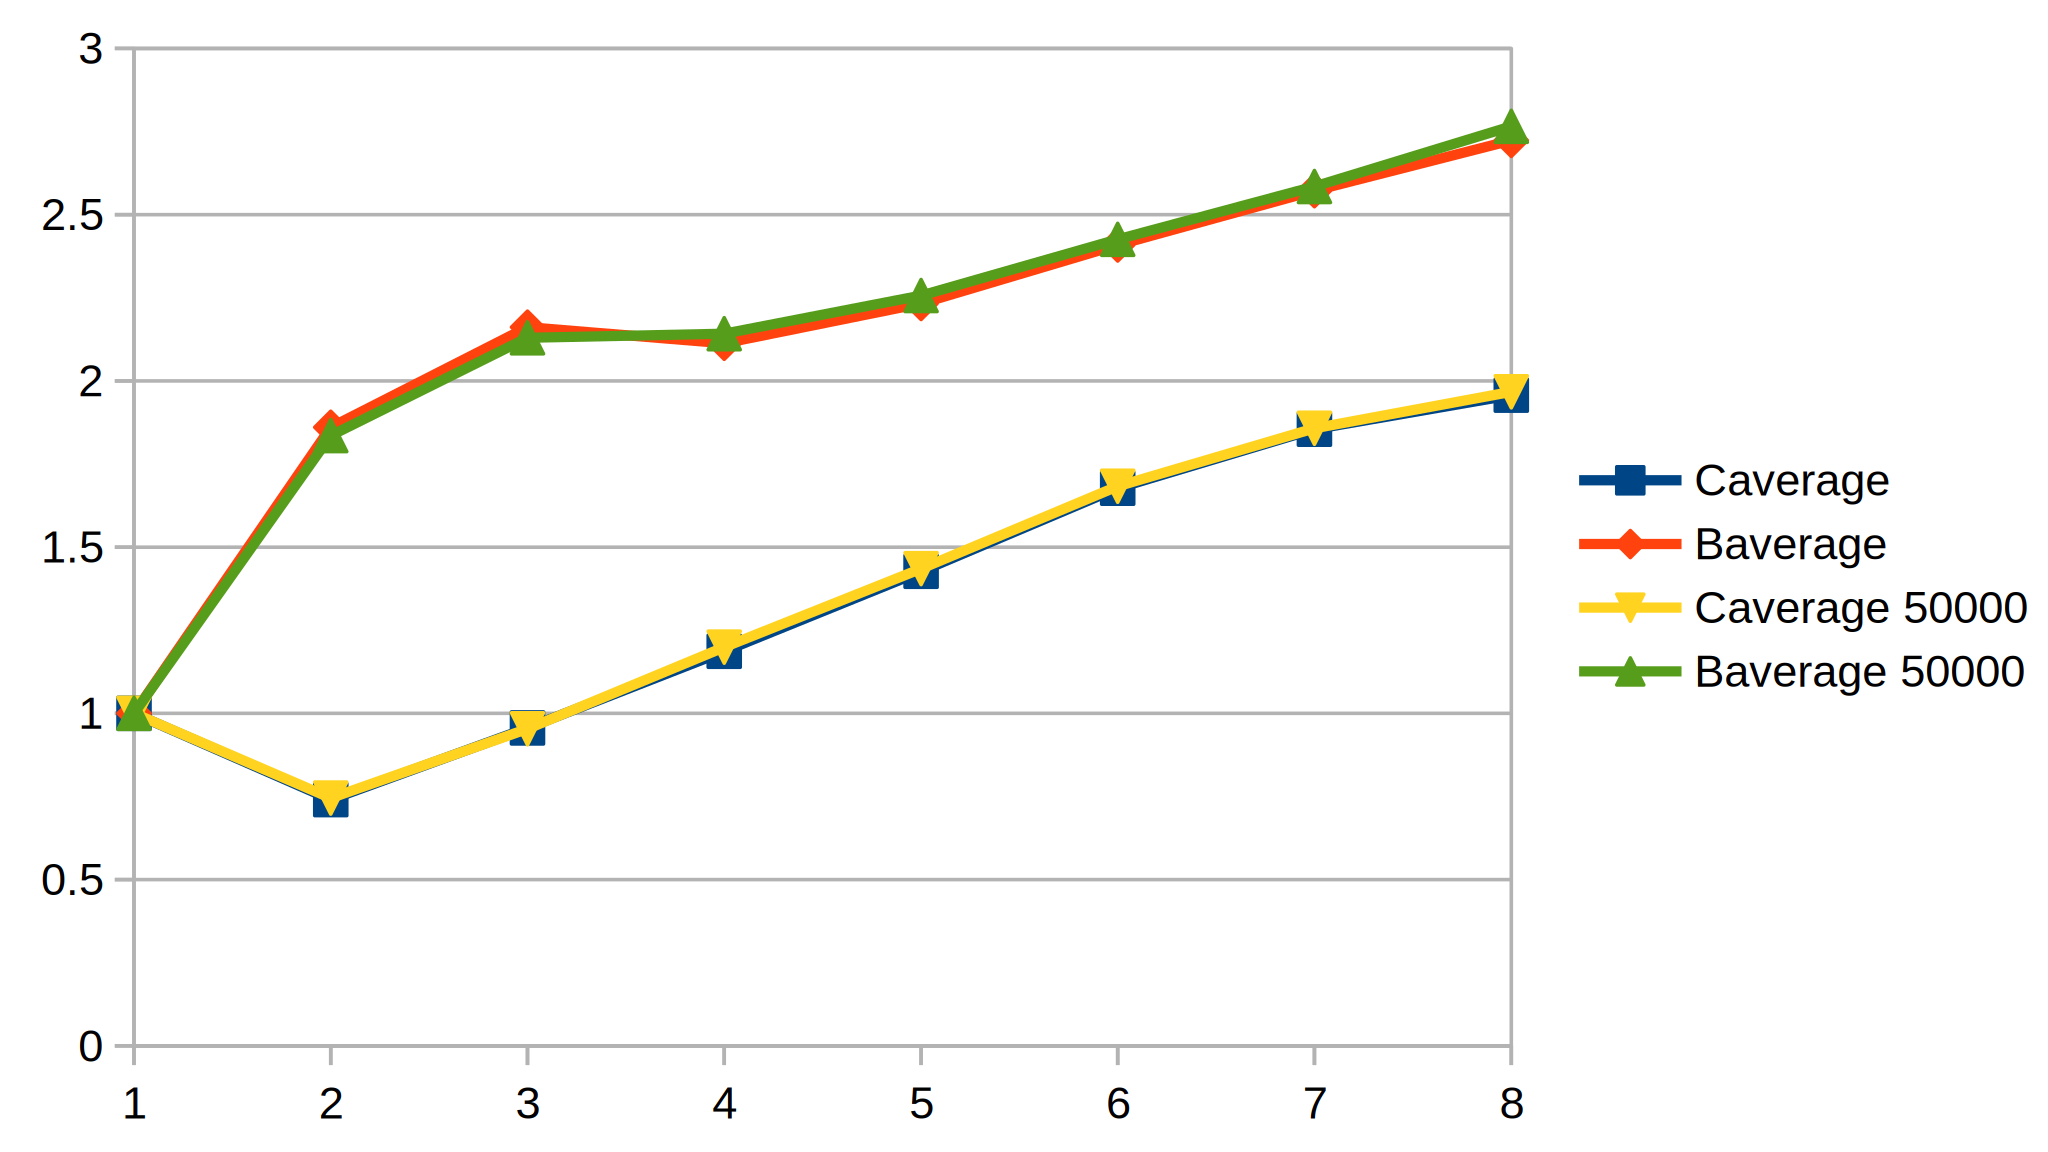
\includegraphics{graphs/graphone}
\caption[Benchmark graph]{Graph showing the speedup of a SME network
  consisting of 20000 and 50000 processes respectively when executed
  for 50000 cycles on an Intel Xeon CPU}
\label{fig:intel-sync}
\end{figure}

\begin{figure}
\centering
\includegraphics{graphs/amd-sync-20000}
\caption[Synchronization-dominated benchmark on AMD cluster]{Benchmark results for a network of 20000 processes running
for 100000 iterations on the AMD cluster}
\label{fig:amd-sync}
\end{figure}


\subsection{Discussion}
We can observe a number of things from the results that can bee seen
in \cref{fig:intel-sync}.  This benchmarks shows the performance of
two different networks, one with 20000 processes and one with 50000
processes. Both networks executed 100000 cycles.

When looking at the graph for our worker-queue model, One thing that
is clearly visible from this benchmark is the overhead produced by the
atomic increment that is required.. This model is doubly penalized
when running the benchmark since we, addition to then time required by
the atomic increment, also need to wait for all of the threads to sync
up at the end of a cycle. What is slightly surprising, however, is the
actual performance that this method shows. It performs significantly
worse when going from one to two threads. The most likely explanation
for this result is CPU optimizations which make atomic updates of a
variable less costly when these updates only occures from one thread.

Our static orchestration model performs quite decently and produces
almost 2x speedup when going from 1 to 2 threads. When adding
additional threads, the speedup decreases, which is expected since the
time spent synchronizing is increased, \fxnote{which manifests as
  dropping CPU-utilization. When running 4 threads, the CPU
  utilization drops to 360\%, unfortunately, I probably wont have time
  to measure or show this}

Common for both of the models, is that the size of the network
executed seems to have no impact on the relative speedups achieved.

Since the Xeon CPU that the benchmarks were performed on only have 4
cores with Hyper Threading, another interesting observation is that
Hyper Threading seems to give a significant additional speedup. One
hypothesis for explaining the cause of this is that branch-prediction
isn't very effective at predicting which functions we're going to call
in our SME network. A branch mis-prediction causes the CPU-pipeline to
be cleared, creating an optimal condition for Hyper Threading to make
use of the empty pipeline-stages\cite{fog2014microarchitecture} While
branch-predictors This hypothesis could be tested by running the
program through a profiler in order to measure the number of
mis-predictions occurring. At this time, these results are not
available.

\Cref{fig:amd-sync} show the results of the smallest version of the
benchmark running on the AMD cluster. The results are significant
worse compared to the results of the Intel Xeon CPU, both in absolute
running times \fxnote{Is it OK to show the numbers?} and
speedup. Early possible explanations was that, due to the extremely
long running time of the benchmark, we were seeing the effects of the
process being moved between CPU-cores. However, the results remained
the same after pinning the threads to CPU-cores placed on the same
NUMA-unit. Thus, the only reasonable explanation explanation is that our
syncronization mechanisms is significantly less optimized on the AMD
CPU compared to the Intel CPU.

Another thing standing out from this benchmark is the huge variability
between the different benchmark runs as shown by the Y-axis error bars.

Due to these very poor initial benchmark results, we didn't attempt
benchmark the synchronization dominated network with different problem
sizes on the AMD-cpu.


\section{Cycle dominated}

\begin{figure}
\centering
\includegraphics{graphs/heavy-ring}
\caption[Synchronization-dominated benchmark on AMD cluster]{Benchmark results for a network of 20000 processes running
for 100000 iterations on the AMD cluster}
\label{fig:heavy-ring}
\end{figure}


In this benchmark, the processes in the network performs a significant
amount work. We expect that this will, to some extent, amortize the
synchronization overhead inherent in the SME model. Combined with the
fact that the individual processes contain no shared state, we
conjecture that this benchmark will scale significantly stronger
than the previous synchronization dominated benchmark that we
performed.

The unit of work being performed by every process in every cycle is
simply to divide a \texttt{long double} number by 3 10000 times. Since
the busses in our SME-implementation only supports transporting
integer values nothing is being done value calculated, but as long as
our workload isn't being optimized away at compilation time this is
irrelevant.

We use floating point numbers as opposed to integer
\fxnote{Yes... good question, Why exactly do we do that?}

The following code is used as workload in our processes
\begin{listing}[H]
\begin{minted}{C++}
private:
  long double n;
  int i;
protected:
void step() {
  n = 533.63556434;
  for (i = 0; i < 10000; i++) {
    n = n/3;
  }
  int val = in->read();
   out->write(++val);
}
\end{minted}
\caption{Code used for generating work in the cycle-dominated
  benchmarks}
\label{lst:cyclecode}
\end{listing}


\section{Discussion}
\fxnote{Not done, points I would like to mention}
\begin{itemize}
\item Static orchestration model (Model 2) provides overall better spewedup
\item Adjusting the ratio of work-to-cycle impacts the speedup that we
  can achieve when using the static orchestration model (as expected)
\item I have no idea what causes the zig-zag patterns
\item The worker-queue model (Model 1) produces identical results
  independent of work-to-cycle. Probably because the single shared
  queue used by all threads makes the threads meet up at the same time 
\item The static-orchestration seems to, for sufficiently large
  workloads, scale liberality, (Yay!)
\end{itemize}


A problem with this benchmark is that the work that we perform can be
performed entirely within the cache of a CPU-core. This allows us to
scale more strongly than when benchmarking a problem which to a larger
extent is limited by memory bandwidth and/or CPU-cache misses.

\section{Uneven workloads}
TODO, if I have time:

Create a mix of the two previous networks such that the statically
orchestrated model will hit its worst-case (very uneven workloads) and
the worker-queue will, by interleaving the small and large processes,
produce better perfomance.


\section{Future works}

More benchmarks:


The results that we have shown, although reasonable, can not be easily
explained by 

\subsection{One-shot process orchestration}
In this model, we orchestrate the processes in our network as soon as
possible after execution start and

\subsection{Monte Carlo orchestration}
In this approach, we simply randomize the order of the processes. The
main advantage of this approach is that is computationally cheap
compared to

\subsection{Optimization-based orchestration}
Another way to orchestrate the processes is to use a


\subsection{Adaptive process orchestration}
The benefits of using a oneshot orchestration approach diminishes when
we execute process networks where the processes performs a variable
amount of work per iteration. In these kinds of networks, CPU-core
load distribution will gradually become uneven and suboptimal as the
network execution progresses. In order to keep this from happening and
maximize CPU-core utilization, we need to monitor process execution
time and core idle time as the network execution progresses. This is
what we refer to s adaptive orchestration. This approach, however
introduces another trade-off that we need to consider. producing an

\subsection{Adaptive Monte Carlo process orchestration}

\subsection{Adaptive Optimization-based process orchestration}



%%% Local Variables:
%%% mode: latex
%%% TeX-master: "master"
%%% TeX-command-extra-options: "-enable-write18"
%%% End:

\chapter{Conculsions}
% We have revealed some of the properties of SME. More real-world usage is still needed in order to decide on the optimal way to implement the network. We have given some options and shown that it is possible to support multiple execution models in the same framework. 

%%% Local Variables:
%%% mode: latex
%%% TeX-master: "master"
%%% TeX-command-extra-options: "-enable-write18"
%%% End:


\printbibliography

\appendix
\section{Compiling and executing}
This section will contain information about how to compile and execute
cppsme 



%%% Local Variables:
%%% mode: latex
%%% TeX-master: "master"
%%% TeX-command-extra-options: "-enable-write18"
%%% End:



\end{document}

%%% Local Variables:
%%% mode: latex
%%% TeX-master: t
%%% TeX-command-extra-options: "-enable-write18"
%%% End:
